\documentclass{article}
\usepackage{fontspec}
\usepackage{xcolor}
\usepackage{amsmath}
\usepackage{amssymb}
\usepackage{unicode-math}
\usepackage[normalem]{ulem} %Underline
\setmainfont{Times New Roman}
\setmathfont{Latin Modern Math}
\setlength\parindent{0pt}

\usepackage{siunitx}
\usepackage{graphicx}
\usepackage[justification=centering]{caption}
\usepackage{pgfplots}
\usepackage{pgfplotstable}
\usepackage{booktabs}
\usepackage{array}
\usepackage{colortbl}
\usepackage{tikz}
\usepackage{makecell}

\begin{document}

\begin{center}
  \textbf{MATH} 131---\textbf{HOMEWORK} 2\\
  \color{red}R\color{teal}icardo
  \color{red}J\color{cyan}.
  \color{red}A\color{teal}cu$\color{red}{\widetilde{\color{teal}\text{n}}}$\color{teal}a\color{black}\\
  \color{teal}(\color{red}862079740\color{teal})\color{black}\\
\end{center}
Q1\quad For each of the following subsets of $\mathbb{F}^3$, determine
whether it is a subspace of $\mathbb{F}^3$:\\

(a) \{$(x_1,x_2,x_3)\in \mathbb{F}^3| x_1 + 2x_2 + 3x_3 = 0$\}\\

It is!\\

\uwave{pf\enskip.}\\
Let $W$ = \{$(x_1,x_2,x_3)\in \mathbb{F}^3| x_1 + 2x_2 + 3x_3 = 0$\}\\

$\forall u,v \in W$: $u = (u_1,u_2,u_3)$ and $v = (v_1,v_2,v_3)$\\
$\Rightarrow u+v = (u_1+v_1,u_2+v_2,u_3+v_3)$\\
$\Rightarrow (u_1 + v_1) + 2(u_2 + v_2) + 3(u_3 + v_3) =\\
u_1 + v_1 + 2u_2 + 2v_2 + 3u_3 + 3v_3 =\\
(u_1 + 2u_2 + 3u_3)+ (v_1 + 2v_2 + 3v_3) =\\ 0 + 0 = 0$ Since $ u,v \in W.$\\
$\Rightarrow u+v \in W$, since $u+v$ satisfies the defining equation
of the set.\\

$\forall k \in \mathbb{F}: ku = (ku_1,ku_2,ku_3)$\\
$0 = k0 = k(u_1 + 2u_2 + 3u_3) = ku_1 + k2u_2 +
k3u_3 = ku_1 + 2ku_2 +
3ku_3$\\
$\Rightarrow ku \in W$
Finally, $0 = 0+2(0)+3(0) \Rightarrow (0,0,0) \in W$.\\

W is a non-empty subset of $\mathbb{F}^3$, closed
under addition and multiplication. So, W is a subspace of
$\mathbb{F}^3$.\enskip$\blacksquare$\\

(b) \{$(x_1,x_2,x_3)\in \mathbb{F}^3| x_1 + 2x_2 + 3x_3 = 4$\}\\

It is not, since $0 + 2(0) + 3(0) = 0 \neq 4$, so (0,0,0) is not in
the set. That means for some $v \neq 0$ in the set, we have  $0v = (0,0,0)$ since 0 $\in \mathbb{F}$ the set can't
be closed under scalar multiplication.\\

(b) \{$(x_1,x_2,x_3)\in \mathbb{F}^3| x_1x_2x_3 = 0$\}\\

Nope! $\forall a,b,c \in \mathbb{F}: a > 0 $ and $ b > 0, $ and $ c >
0, 0 \in \mathbb{F}$.
$(a,b,0)$ is in the set since $ab0=0$, and $(0,0,c)$ is also in
the set, since $0^2c=0$. But, since $(a,b,0) + (0,0,c) = (a,b,c)$,
$(a,b,c)$ is not in the set because $abc > 0$. So the set is not
closed under addition.\\

\newpage
Q2\quad Prove or give a counterexample:
The intersection of any two subspaces of V is a subspace.\\

\uwave{pf\enskip.}\\
$\forall W_1,W_2: W_1,W_2$ are subspaces of $V$:\\
$W_1 \cap W_2 = \{w | w \in W_1$and$ w\in W_2\}$\\

$W_1$ is a subspace of V$ \Rightarrow 0 \in W_1 \Rightarrow
0 \in W_1 \cap W_2$\\
$\Rightarrow W_1 \cap W_2$ is not empty\\

$\forall k \in \mathbb{F}: $Let $u,v \in W_1 \cap W_2$:\\
$\Rightarrow u \in W_1$ and $ v \in W_1 \Rightarrow k(u+v) \in W_1$ Since
$W_1$ is a subspace of $V$\\
$\Rightarrow u \in W_2$ and $ v \in W_2 \Rightarrow k(u+v) \in W_2$ Since
$W_2$ is a subspace of $V$\\
$k(u+v) \in W_1$ and $k(u+v) \in W_2 \Rightarrow k(u+v) \in W_1 \cap
W_2$\\
$\Rightarrow W_1 \cap W_2$ is closed under addition and multiplication.\\
So, $W_1 \cap W_2$ is a subspace of $V$ $\blacksquare$\\

Q3\quad Prove or give a counterexample: If $U_1$ , $U_2$ and $W$ are subspaces
of $V$ such that $U_1 + W = U_2 + W$, then $U_1 = U_2$.\\

\uwave{pf\enskip.}\\
$\forall U_1, U_2, W: U_1, U_2, W$ are subspaces of $V$\\
$U_1 + W = \{u_1 + w | u_1 \in U_1 $ and $ w \in W\}$\\
$U_2 + W = \{u_2 + w | u_2 \in U_2 $ and $ w \in W\}$\\
$U_1 + W = U_2 + W \\ \Rightarrow\{u_1 + w |\enskip u_1 \in U_1 $ and $ w
\in W\} = \{u_2 + w |\enskip u_2 \in U_2 $ and $ w \in W\}$\\
Since $W$ is a subspace of $V$, $0 \in W$, so I can:\\
Let $X \subset U_1 + W: X = \{u_1 + 0 | u_1 \in U_1$ and $0 \in W \}$\\
and $Y \subset U_2 + W: Y = \{u_2 + 0 | u_2 \in U_2$ and $0 \in W \}$\\
So, restricting both sets to the same element of $W$, namely $0
\Rightarrow X=Y$.\\
Now, $\forall u_1 + 0 \in X: u_1 + 0 = u_1 \Rightarrow X = U_1$\\
, and $\forall u_2 + 0 \in Y: u_2 + 0 = u_2 \Rightarrow Y = U_2$\\
So, if $U_1 + W = U_2 + W$, then $U_1 = U_2$ $\blacksquare$\\

\newpage
Q4\quad Give an example of a nonempty subset $U$ of $\mathbb{R}^2$ such that $U$ is
closed under addition, but $U$ is not a subspace of $\mathbb{R}^2$.\\

\color{gray}$U$\color{black} = \{$(x,y)\in \mathbb{R}^2 |\enskip y \geq 0$\}\\
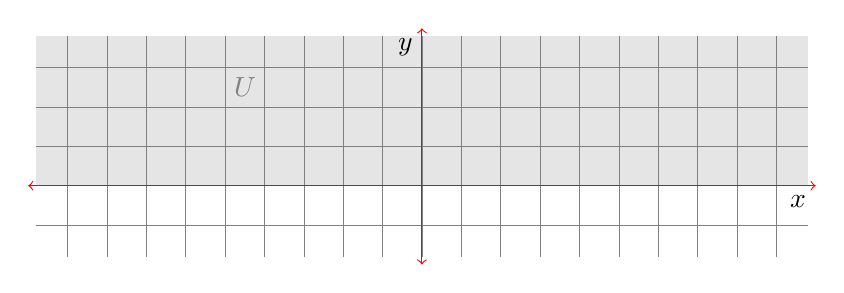
\begin{tikzpicture}
  \fill[black!10!white] (0.1,0.9) rectangle (9.9,-1);
  \draw[step=0.5 cm,gray,very thin] (0.1,0.9) grid (9.9,-1.9);
  \draw [<->,red] (5,1) -- (5,-2);
  \node [below left] at (5,1) {$y$};
  \draw [<->,red] (0,-1) -- (10,-1);
  \node [below left] at (10,-1) {$x$};
  \node[below right,black!50!white] at (2.5,0.5) {$U$};
\end{tikzpicture}\\
Let $(x_1,y_1),(x_2,y_2) \in U$: Since there's no restriction on x,
$x_1+x_2$ is ok, now since $y_1$ and $y_2$ are bigger than or equal to
0, $y_1+y_2$ is greater than or equal to 0. So $U$ is closed under
addition. But, $\exists -1 \in \mathbb{F}: -1(x_1,y_1) = (-x_1,-y_1)$
Since $y_1$ is positive, $-y_1$ is negative. That means $(-x_1,-y_1)
\notin U$, so it's not closed under, scalar multiplication.\\

Q5\quad Prove or disprove:
$U = \{f ∈ R[x] | f^{\prime\prime}(x)= 0\}$
is a subspace of $\mathbb{R}[x]$.\\

\uwave{pf\enskip.}\\
$\forall k \in \mathbb{F}: \forall f,g \in U:$\\
$f^{\prime\prime}(x)= 0 \Rightarrow f^{\prime}(x) = \int 0\enskip ds =
C \in \mathbb{F} \Rightarrow f(x) = \int C dx = Cx + E_1 $\\
Similarly $g(x) = Dx +E_2,$ some $ D,E_1,E_2 \in \mathbb{F}$.\\

$\Rightarrow k(f+g) (x) = k(f+g(x)) = k(f(x) +g(x))
\\ = k(Cx + E_1 + Dx + E_2) = k(C+D) x +k(E_1 + E_2)\\ \Rightarrow
[k(f+g)]^{\prime} (x) = k(C+D) \in \mathbb{F} \Rightarrow
[k(f+g)]^{\prime\prime}(x) = 0$.\\

The zero function $0(x) = 0$, has $0^{\prime\prime}(x) = 0$.\\

So, $U$ is a non-empty subset of $\mathbb{R}[x]$, with the
coefficients of higher powers of $x$ set to $0$, that is closed under
addition and multiplication.\blacksquare\\
\newpage
Q6\quad For each of the following subset of Mat$_{3×3}(\mathbb{F})$, determine whether
it is a subspace of Mat$_{3×3}(\mathbb{F})$. If it is a subspace,
prove it. If it is not a subspace, explain why.\\

(1) $S_1 = \{A \in $Mat$_{3×3}(\mathbb{F}) |\enskip $tr$ A = 0\}$\\

\uwave{pf\enskip.}\\
$\forall A,B \in S_1: A = (a_{ij})$ and $B = (b_{ij})$
$\Rightarrow A + B = (a_{ij} + b_{ij}) \\
\Rightarrow$ tr $A + B =  \sum_{i=1}^3 a_{ii} + b_{ii} = \sum_{i=1}^3
a_{ii} + \sum_{i=1}^3 b_{ii} = 0 + 0 = 0$\\
$\Rightarrow A + B \in S_1$\\

$\forall k \in \mathbb{F}: kA = (ka_{ij})$\\
$\Rightarrow$  tr $kA = \sum_{i=1}^3 ka_{ii} = k\sum_{i=1}^3 a_{ii} =
k0 = 0$\\
$\Rightarrow kA \in S_1$\\

$0_{3x3} \in$ Mat$_{3x3}(\mathbb{F})$: $0_{3x3} = (z_{ij}) := \forall
z_{ij} \in 0_{3x3}: z_{ij} = 0$\\
$\Rightarrow$ tr $0_{ij} = \sum_{i=1}^3 z_{ij} = \sum_{i=1}^3 0 = 0$\\
$\Rightarrow 0_{ij} \in S_1$\\

$\Rightarrow S_1$ is a non-empty subset of Mat$_{3×3}(\mathbb{F})$, that is
closed under addition and scalar multiplication.\\
So, $S_1$ is a subspace of Mat$_{3×3}(\mathbb{F})$ $\blacksquare$\\

(2) $S_2 = \{A \in $Mat$_{3×3}(\mathbb{F}) |\enskip $det$ A = 0\}$\\

$
\begin{vmatrix}
  1&0&0\\
  0&1&0\\
  0&0&0
\end{vmatrix}=0
$
and
$\begin{vmatrix}
  0&0&0\\
  0&0&0\\
  0&0&1
\end{vmatrix}=0$\\

But,
$\\
\begin{vmatrix}
\begin{pmatrix}
  1&0&0\\
  0&1&0\\
  0&0&0
\end{pmatrix}
+
\begin{pmatrix}
  0&0&0\\
  0&0&0\\
  0&0&1
\end{pmatrix}
\end{vmatrix}
=
\begin{vmatrix}
  1&0&0\\
  0&1&0\\
  0&0&1
\end{vmatrix}
=1
$\\

So, $S_2$ is not closed under addition.\\
Note: here |\_|:= det (\_)
\end{document}

%%% Local Variables:
%%% mode: latex
%%% TeX-master: t
%%% End:
